\documentclass[a4paper,8pt]{article}

% Packages for formatting
\usepackage{geometry}
\usepackage{float}
\usepackage{array}
\usepackage{lipsum}
\usepackage{cite}
\geometry{margin=1in}
\usepackage{booktabs}
\usepackage[table]{xcolor}
\usepackage{graphicx}
\usepackage{tabularx}
\usepackage{longtable}
\usepackage{amsmath}
\usepackage{caption}
\captionsetup{font=normalsize} % This will fix captions being resized
\usepackage[colorlinks=true, linkcolor=blue, urlcolor=blue, citecolor=blue]{hyperref}
\usepackage{tocloft}

\title{Bill of Materials (BOM) Explanation}
\author{ Pontus Svensson / RoboCup }
\date{\today}

\begin{document}

  \maketitle

  \tableofcontents

  \newpage

  \section{Introduction}

  This document provides an explanation of the Bill of Materials (BOM)
  we want to use in the project. Each component listed in the BOM is
  described in detail, including its purpose and other relevant
  specifications.

  \section{Component Overview}

  The table below outlines the components used in this project along
  with their purpose and additional information.
  \begin{center}
    \begin{longtable}{|p{3cm}|p{3cm}|p{3cm}|p{1cm}|p{3cm}| }
      \caption{Component Descriptions for the Project}
      \\ \hline \rowcolor{gray!50} \textbf{Component} & \textbf{Description} & \textbf{Purpose} & \textbf{\#} & \textbf{á price (price per robot) SEK}\\ \endhead \hline

      \rowcolor{gray!50} \textbf{Total price for 1 robot} & \textbf{8440.9} \endlastfoot \hline

      DF45L024048-A & Brushless direct current (BLDC) motor with integrated hall sensors for the wheels & Used to spin the wheels of the robot. & 4 & 830.4 (3273.60)\\ \hline 
      Hobbywing FPV XRotor 3110 900KV & Brushelss DC motor & High revolutions per minute (RPM) motor used to control the dribbler. & 1 & 175.20 (175.20) \\ \hline 
      B-G431B-ESC1 & BLDC motor driver & Motor driver with embedded $\mu\text{Controller}$ current sensing and hall sensing to form a closed-loop control algorithm & 5 & 208.96 (1044.8) \\ \hline 
      NUCLEO-H723ZG & $\mu\text{Controller}$ & Computational power and real-time processing capabilities, supports $\mu\text{ROS}$ & 1 & 322.58 (322.58) \\ \hline 
      Raspberry Pi 4 Model B/8GB & Single-board computer & Processing camera input and performing local path planning & 1 & 979 (979) \\ \hline
      SX1280IMLTRT & Radio frequency (RF) transceiver & Used to transmit data over 2.4Ghz network & 1 & 75.44 (75.44) \\ \hline 
      SKY66122-11 & Integrated front-end-moduel (FEM) & Simplified integration with the RF circuit & 1 & 40.48 (40.48) \\ \hline 
      6s 1300mAh -120C - GNB HV XT60 & LiPo-battery & Used to power the robot & 1 & 351.20 (351.20) \\ \hline 
      LT3750 & Charging controller for the capacitors of the kicker & Charge controller for the kicker circuit & 1 & 146.93 (146.93)\\ \hline 
      iC-PX2604 + PX01S 26-30 & Wheel encoders & Will be used for odometry of the robot & 4 & 224.40 (897.60) \\ \hline 
      WSEN-ISDS 6 Axis IMU & 6-DoF IMU & Will be used for odometry of the robot & 10 & N/A\\ \hline 
      Raspberry Pi Camera-module 3 & Camera & Provide images in front of the robot to detect the ball and obstacles & 1 & 369 (369) \\ \hline 
      IR Break Beam Sensor - 5mm LEDs & Infrared (IR) sensor & Used to detect if the ball is close to the robot & 1 & 99 (99) \\ \hline 
      JST 6B-PH-K-S & Connector & Hall sensor connector from the motor & 4 & 3.85 (15.4) \\ \hline 
      JST B5P-VH & Connector & Motor connector & 4 & 4.06 (16.24) \\ \hline 
      Connectors & Passive component & Supplied by Würth & N/A & N/A \\ \hline 
      Shaft hub with clamping bracket 4mm & Coupler & Couple the wheels with the motor shaft & 4 & 139 (556) \\ \hline 
      Bearings & Bearings & Make the roller spin (dribbler) & 2 & 18 (36)\\ \hline 
      Resistors & Passive component & Supplied by Würth or 326 & N/A & N/A \\ \hline 
      Capacitors & Passive component & Supplied by Würth or 326 & N/A & N/A \\ \hline 
      Voltage regulators & DC/DC buck converters & Supplied by Würth & N/A & N/A \\ \hline 
      Solenoid & Solenoid & Supplied by MDU & 1 & N/A \\ \hline 
      PCB & Printed circuit board (PCB) & The students will supply any custom PCB designed & 2 & N/A\\ \hline
      LM74500\break-QDDFRQ1 & Reverse polarity protection & Used to
      protect against wrong polarity connections & 1 & 16.45 (16.45) \\ \hline 
      BUK9Y8R5-80EX & N-channel mosfet & Used with the LM74500\break-QDDFRQ1 & 1 & 17.95 (17.95) \\ \hline 
      SMBJ58A & TVS+ & ESD protection diode, used in reverse polarity circuit & 1 & 4.5 (4.5) \\ \hline 
      SMBJ26A & TVS- & ESD protection diode, used in reverse polairiy circuit & 1 & 3.53 (3.53) \\ \hline
    \end{longtable}
  \end{center}

  \section{Reason for component choice}

  \subsection{DF45L024048-A}

  % SSL robot motor characteristic
  During competition a SSL-robot is most of the time accelerating
  \cite{francaRob^oCInSmallSize}. Having a motor which can provide
  sufficient torque at any given speed is crucial.

  % DF45L024048-A introduction
  The DF45L024048-A BLDC motors provides a good tradeoff between torque
  and RPM, with integrated hall sensors. The sensors detect the position
  of the rotor relative to the stator which gives the ability to control
  the motors using commutation. The motor controller uses the signals
  from the hall sensors to determine the exact timing for switching the
  current in the stator windings. This gives a smooth motor operation
  while maximizing torque output.

  % Other considerations
  We also have to take the size of the motor into account. Having to
  large footprint on the motors would cause the kicker (solenoid) to not
  fit in the chassi. Using a general 5010 sensorless drone motor could
  be used as demonstrated by \cite{veeraghanta2024TeamDescription} but
  this motor would require a more sophisticated ESC which would take a
  lot of time to develop and manufacture. The problem with searching for
  5010 drone motors is that they are most websites does not show the
  full torque graph, they primarly show the torque when the motor is
  already spinning at $40\%$ and above. Therefore finding a 5010 drone
  motor with adequate torque at low speeds is deceptively difficult.

  % Provide sources for my claims
  Using hall sensors is a common method utilized by several teams and
  proven to be a winning concept \cite{ryllExtendedTeamDescription}\cite{abiyevNEUIslandersTeamDescription}\cite{wuCompilationErrorTeam}\cite{francaRob^oCInSmallSize}.

  % Dribbler

  \subsection{Hobbywing FPV XRotor 3110 900KV}

  % Dribbler requirements
  The requirements for the dribbler motor is that it can reach high RPM
  (around $10\:000\text{ RPM}$). No feedback is implemented for the
  dribbler motor, due to the timeframe of the project we will not have
  time to implement a control algorithm for the dribbler.

  % Motor driver

  \subsection{B-G431B-ESC1}

  % Sensorless controller hiccups
  A sensorless controller requires that the BLDC motor produce a
  measurable back electromotive force (EMF) so the controller can
  determine the position of the rotor and therefore cannot provide
  smooth commutation at start up and low speeds.
  \cite{roweInstrumentationControlHigh2012}

  % Introduction to B-G431B-ESC1
  The chosen electronics speed controller (ESC) has an STSPIN32F0A
  system in package chip which has an integrated STM32 processor with
  hall sensor decoding logic and current sensing capabilities. This
  makes this ESC a good fit with the DF45L024048-A BLDC motor.

  % STSPIN32F0A
  The STSPIN32F0A chip is a common choice for controlling BLDC motors in
  the SSL competitions which has been proven to be reliable and
  succesful
  \cite{ryllExtendedTeamDescription}\cite{abousaleh2024TeamDescription}

  % PID system
  A PID system can be implemented on the chip to allow for precise
  movement and rapid acceleration which is critical to make fast
  directions changes.

  % Implementation plan of the PID
  The B-G431B-ESC1 will receive a desired velocity, to use this with in
  a PID system the RPM of each motor is required. The RPM will be
  retrieved by measuring the number of pulses from the hall sensors and
  calculate the time between them or by using the optical wheel
  encoders.

  % Size and weight
  The size and weight of the ESC does also have to be taken in
  consideration, the B-G431B-ESC1 has a small footprint with a
  relatively low weight $286\text{g}$. With all the components
  integrated on one board will make the assembly process easier and
  reduce any external components e.g. hall sensing or mosfets. The
  programming for the integrated STM32 is done using STM32 Motor Control
  Software Development Kit which is a graphical programming environtment
  from ST.

  \subsection{NUCLEO-H723ZG Microcontroller}

  The \text{NUCLEO-H723ZG} is a development board based on the
  STM32H723ZG chip, it comes with all necessary peripheral communication
  UART, SPI, I2C and CAN. The STM32H723ZG features an ARM Cortex-M7 core
  operating at up to 480 MHz, providing good processing power for
  handling multiple real-time tasks required in our application.

  Additionally, the STM32 series is widely adopted in RoboCup
  competitions, including the \textbf{Small Size League (SSL)} \cite{ryllExtendedTeamDescription}\cite{zhaoZJUNlictExtendedTeam}\cite{wuCompilationErrorTeam}.
  This widespread use underscores its reliability and effectiveness in
  competititions.

  To manage the various tasks and ensure smooth operation of our robot,
  we will implement a control architecture using \textbf{micro-ROS} in
  combination with \textbf{FreeRTOS} on the NUCLEO-H723ZG.

  \textbf{FreeRTOS} is a real-time operating system that provides task
  scheduling and resource management. Implementing FreeRTOS on the
  NUCLEO-H723ZG allows us to handle multiple concurrent tasks
  efficiently, such as sensor data processing, motor control, and
  communication with other system components.

  This also aligns with the collaboration with Universidad de Antioquia,
  since they will use FreeRTOS to program the ESP32-S3.

  \subsection{Raspberry Pi 4 Model B/8GB}

  It is important to accurately detect the ball and other robots in a
  timely manner, therefore we have decided to use a camera which image
  input will be processed by the Raspberry Pi 4. The Raspberry pi has
  been extensively used in the SSL competitions for this purpose
  \cite{ommerExtendedTeamDescription}\cite{satoGreenTea2024Team}.

  The Raspberry Pi 4 was also chosen to be able to run the DWA path
  planning algorithm, due to the timeframe of this project, implementing
  DWA by ourself would require too much time.

  \subsection{SX1280IMLTRT + SKY66122-11}

  To obtain a reliable connection to the team server, we have opted to
  use the SX1280IMLTRT RF transceiver with the SKY66122-11
  front-end-module.

  This implementation has been proven succesful by several teams \cite{ryllExtendedTeamDescription}\cite{barretoRoboIMEIgnitingInnovation}.

  However, one drawback is that the components require a custom made
  PCB. This will be solved by creating one mainboard with connectors to
  our components, battery, motors, sensors and the NUCLEO-H723ZG. This
  will enable a modular design where components can be swapped.

  \subsection{iC-PX2604 + PX01S 26-30}

  This wheel encoder comes as a complete module which will be easy to
  integrate and in combination with the NUCLEO-H723ZG the resolution of
  the encoder is increased. Since we also have a quotation at a
  reasonable price we have chosen to use this encoder.

  \subsection{WSEN-ISDS 6 Axis IMU}

  Ther IMU we have chosen is supplied free of charge from Würth
  electronics. It communicates using I2C or SPI which both are available
  on the NUCLEO-H723ZG.

  \subsection{Raspberry Pi Camera-module 3}

  The Raspberry Pi camera-module 3 is chosen because its seamless
  integration with the Raspberry Pi 4.

  \subsection{IR Break Beam Sensor - 5mm LEDs}

  The IR Break Beam sensor will be connected using GPIO pins on the
  NUCLEO-H723ZG with a pull-up resistor.

  \subsection{Connectors}

  Connectors for the main PCB board will be supplied by Würth
  electronics.

  \subsection{Shaft hub with clamping bracket 4mm}

  From our research teams have noticed that if the coupling between the
  motorshaft and wheels does not have a good fit, the shaft will start
  to release tiny metal dust which will be collected by the hub of the
  BLDC motor.

  Therefore we have chosen to use this clamp to ensure the coupling is
  secure.

  \subsection{Bearings}

  Bearings used for the roller.

  \subsection{Resistors}

  Any Passive components required will be supplied by Würth electroncis
  or if we can find it in 326.

  \subsection{Capacitors}

  Any Passive components required will be supplied by Würth electroncis
  or if we can find it in 326.

  \subsection{Voltage regulators}

  The voltage regulators will be used to ensure our components reveice
  the correct voltages, 3.3V, 5V, 12V will be integrated on the custom
  PCB.

  The voltage regulators was supplied by Würth electronics.

  \subsection{Solenoid}

  A custom made solenoid would be preferred, but due to time the
  solenoid we will use is a generic solenoid for starting car engines.
  Supplied by MDU.

  \subsection{PCB}

  As some of our components require a custom PCB, we will design two
  PCBs. A mainboard and a kicker-board, the main board will host
  connectors for the battery, motors, NUCLEO-H723ZG and pin headers for
  powering the Raspberry Pi. The mainboard will also host the RF
  transceiver, IMU and voltage regulators.

  \section{Hardware Architecture}

  Figure\Figure~\ref{fig:hardware_architecture} depicting the hardware
  architecture of the proposed robot.

  \begin{figure}[H]
    \begin{center}
      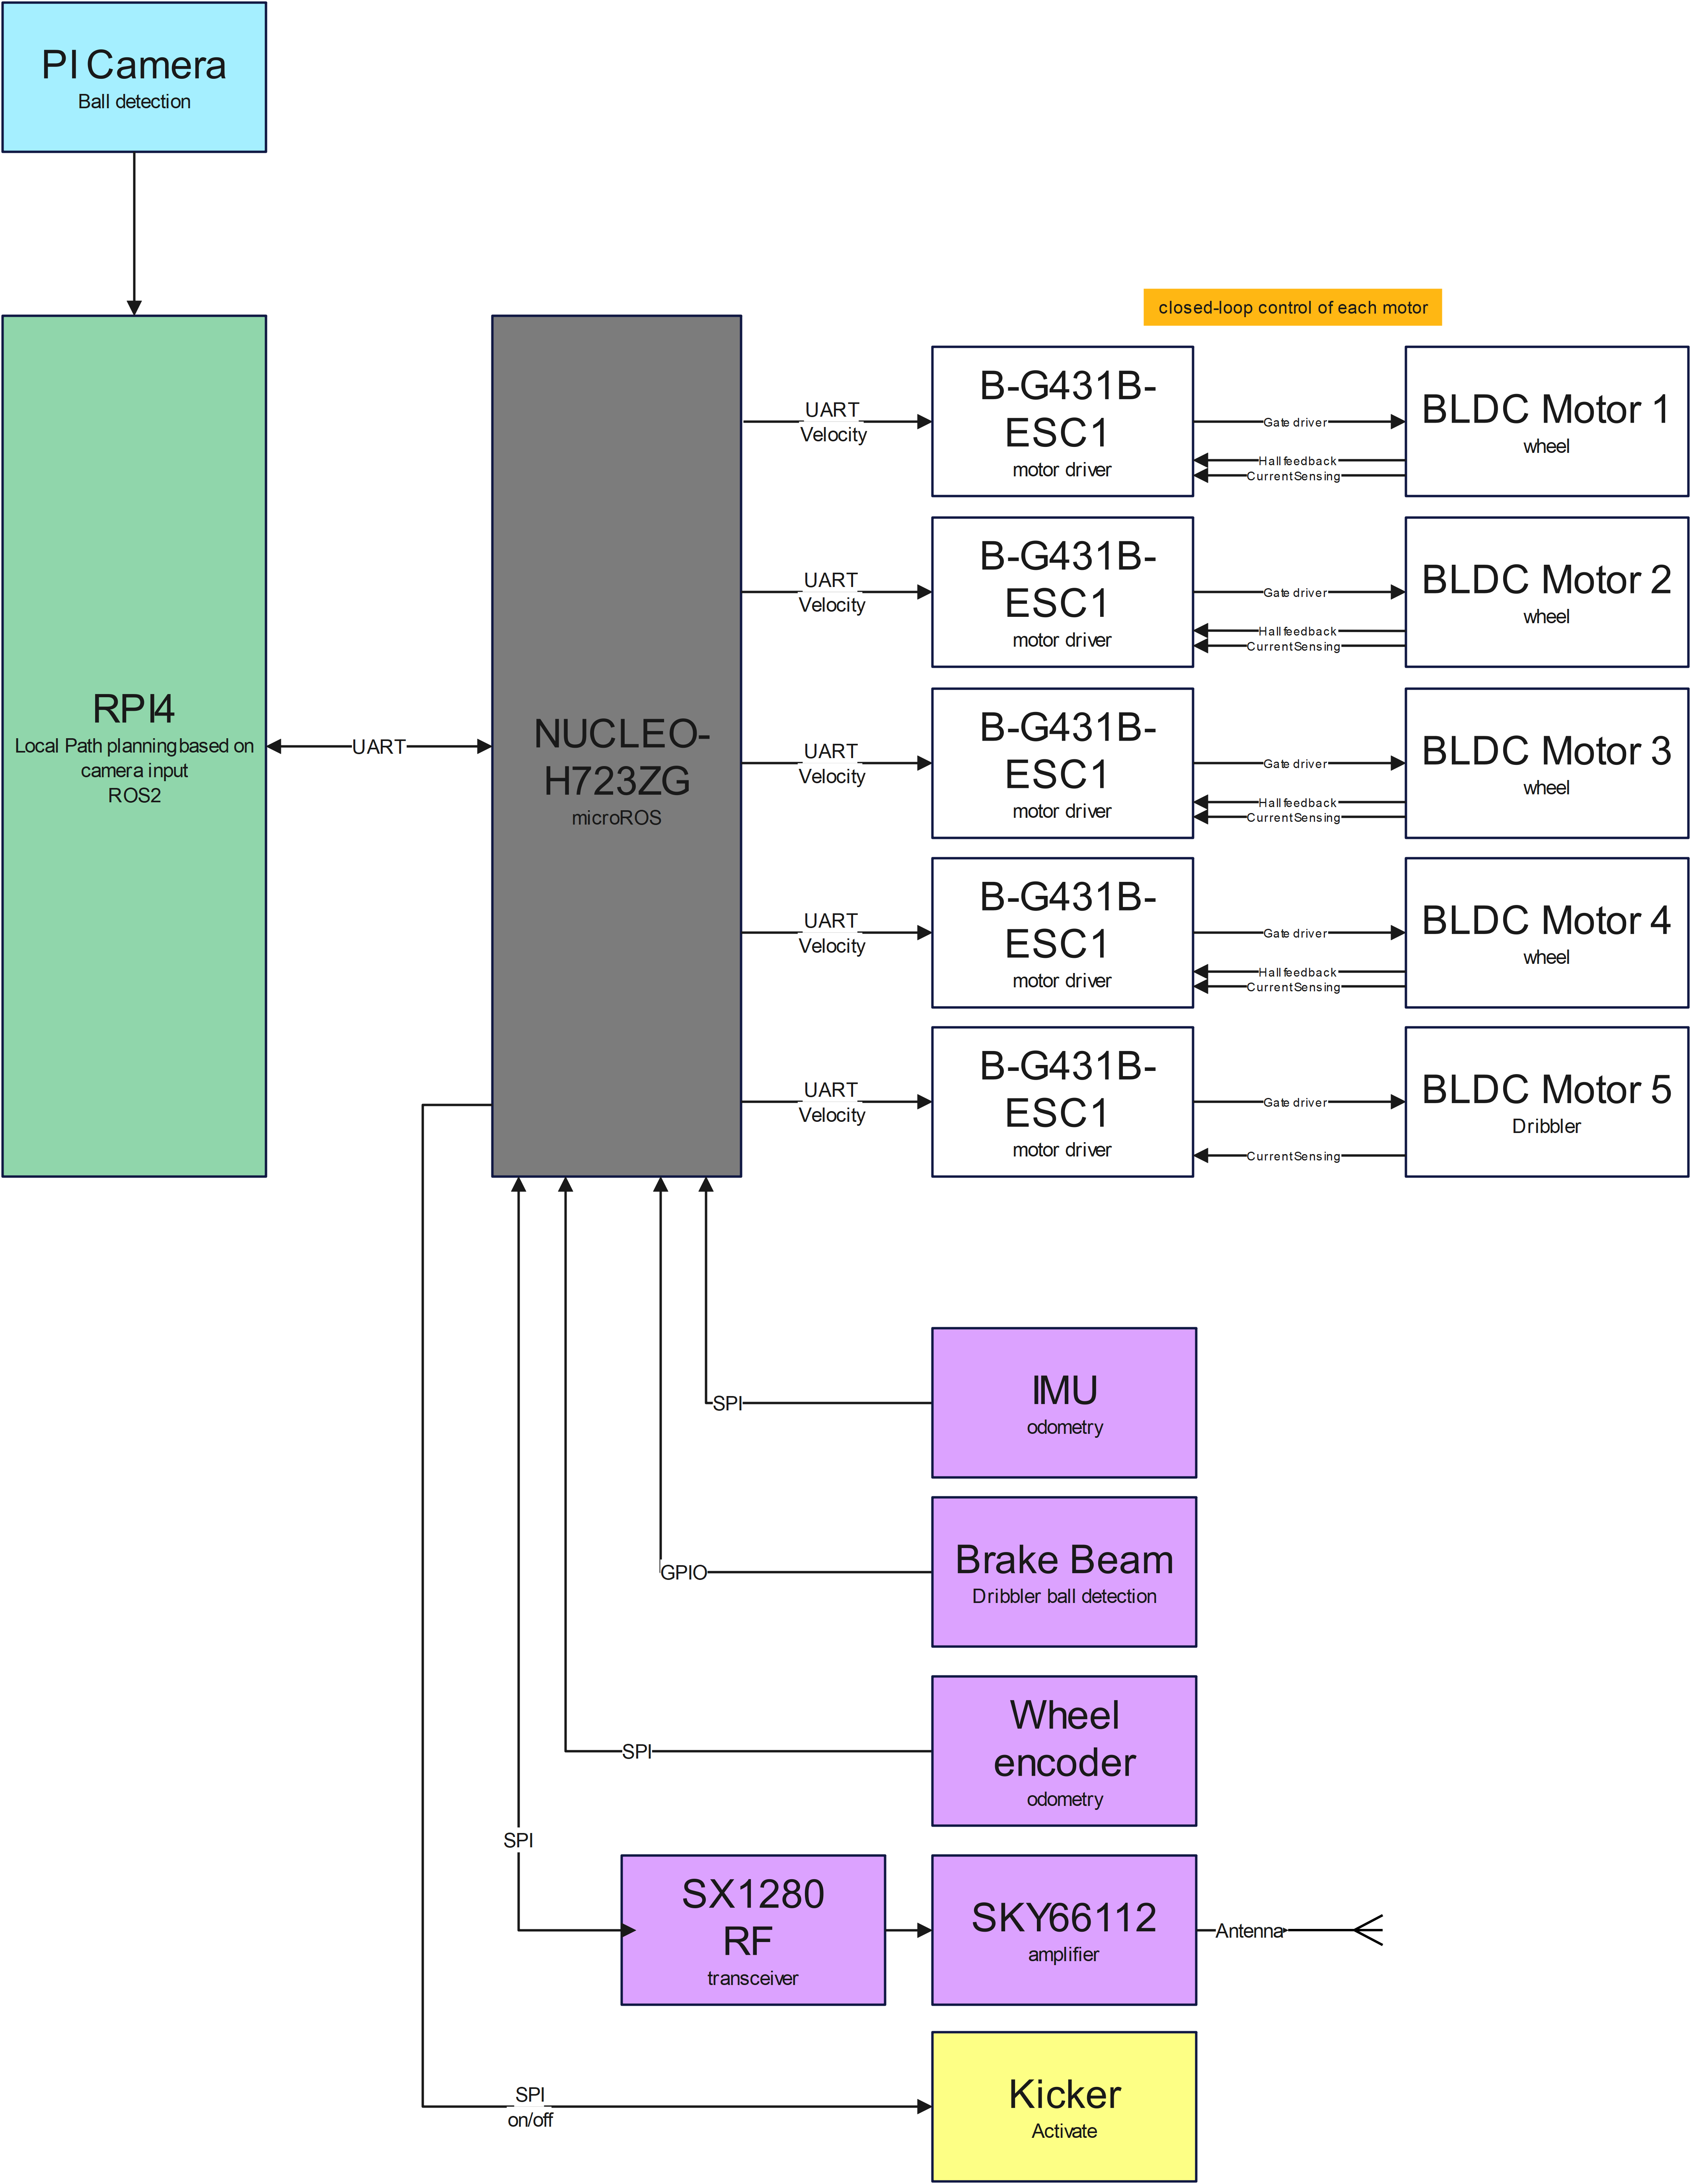
\includegraphics[width=0.5\textwidth]{Hardware_architecture.png}
    \end{center}
    \caption{Hardware Architecture}
    \label{fig:hardware_architecture}
  \end{figure}

  \section{Hardware Interface}

  \section{Alternative BOM that has equal components to UdeA
    Collaboration}

  \begin{small}
    \begin{longtable}{|p{3cm}|p{3cm}|p{3cm}|p{1cm}|p{3cm}| }
      \caption{Alternative BOM} \\ \hline 
      \rowcolor{gray!50} \textbf{Component} & \textbf{Replaces} & \textbf{Purpose} & \textbf{\#} & \textbf{á price (price per robot) SEK}\\ \endhead \hline

      \rowcolor{gray!50} \textbf{Total price for 1 robot} & \textbf{8440.9} \endlastfoot \hline

      MN5208 Navigator Type UAV Multi-Motor KV340 & DF45L024048-A & BLDC motor & 4 & 1027.32 (4109.28)\\ \hline
      Hobbywing FPV XRotor 3110 900KV & N/A & High revolutions per minute (RPM) motor used to control the dribbler. & 1 & 175.20 (175.20) \\ \hline 
      B-G431B-ESC1 & N/A & Motor driver with embedded $\mu\text{Controller}$ current sensing and hall sensing to form a closed-loop control algorithm & 5 & 208.96 (1044.8)\\ \hline 
      ESP32-S3-DevKitC-1-N32R8V & NUCLEO-H723ZG & Chosen by UdeA & 1 & 181.82 (181.82) \\ \hline 
      Raspberry Pi 4 Model B/8GB & N/A & Processing camera input and performing local path planning & 1 & 979 (979) \\ \hline 
      SX1280IMLTRT & N/A & Used to transmit data over 2.4Ghz network & 1 & 75.44 (75.44) \\ \hline 
      SKY66122-11 & N/A & Simplified integration with the RF circuit & 1 & 40.48 (40.48) \\ \hline 
      6s 1300mAh -120C - GNB HV XT60 & N/A & Used to power the robot & 1 & 351.20 (351.20) \\ \hline 
      LT3750 & N/A & Charge controller for the kicker circuit & 1 & 146.93 (146.93)\\ \hline
      AS5600-SO\_EK\_AB & iC-PX2604 + PX01S 26-30 & Will be used for odometry of the robot & 4 & 224.40 (897.60) \\ \hline 
      WSEN-ISDS 6 Axis IMU & N/A & Will be used for odometry of the robot & 10 & N/A\\ \hline 
      Raspberry Pi Kameramodul 3 & N/A & Provide images in front of the robot to detect the ball and obstacles & 1 & 369 (369) \\ \hline 
      IR Break Beam Sensor - 5mm LEDs & N/A & Used to detect if the ball is close to the robot & 1 & 99 (99) \\ \hline 
      Generic motor connectors & JST B5P-VH & Motor connector & 4 & 4.06 (16.24) \\ \hline
      Connectors & Passive component & Supplied by Würth & N/A & N/A \\ \hline 
      Shaft hub with clamping bracket 4mm & Coupler & Couple the wheels with the motor shaft & 4 & 139 (556) \\ \hline 
      Bearings & Bearings & Make the roller spin (dribbler) & 2 & 18 (36)\\ \hline
      Resistors & Passive component & Supplied by Würth or 326 & N/A & N/A \\ \hline 
      Capacitors & Passive component & Supplied by Würth or 326 & N/A & N/A \\ \hline 
      Voltage regulators & DC/DC buck converters & Supplied by Würth & N/A & N/A \\ \hline 
      Solenoid & Solenoid & Supplied by MDU & 1 & N/A \\ \hline 
      PCB & Printed circuit board (PCB) & The students will supply any custom PCB designed & 2 & N/A\\ \hline 
      LM74500\break-QDDFRQ1 & Reverse polarity protection & Used to protect against wrong polarity connections & 1 & 16.45 (16.45) \\ \hline 
      BUK9Y8R5-80EX & N-channel mosfet & Used with the LM74500\break-QDDFRQ1 & 1 & 17.95 (17.95) \\ \hline 
      SMBJ58A & TVS+ & ESD protection diode, used in reverse polarity circuit & 1 & 4.5 (4.5) \\ \hline 
      SMBJ26A & TVS- & ESD protection diode, used in reverse polairiy circuit & 1 & 3.53 (3.53) \\ \hline
    \end{longtable}
  \end{small}

  \section*{Conclusion}

  This document serves as a reference for understanding the role of each
  component in the project. For any further technical details, please
  refer to the respective datasheets provided by the manufacturers.

  \newpage
  \bibliographystyle{IEEEtran} \bibliography{DVA490_DVA474}
  % Point to your .bib file (without the .bib extension)
\end{document}
